
%%%%%%%%%%%%%%%%%%%%%%%%%%%%%%%%%%%%%%%%%%%%%%%%%%%%%%%%%%%%%%%%%%
% Artigo segundo as normais mais atualizadas da ABNT
% Adaptado do projeto ABNTeX2 (que nao esta totalmente sincronizada com as normas da ABNT)
%%%%%%%%%%%%%%%%%%%%%%%%%%%%%%%%%%%%%%%%%%%%%%%%%%%%%%%%%%%%%%%%%%
\documentclass[article,12pt,oneside,a4paper,english,brazil,sumario=tradicional]{abntex2}
% Pacotes usados
\usepackage{times}%Usa a fonte Latin Modern
\usepackage[T1]{fontenc}%Selecao de codigos de fonte.
\usepackage[utf8]{inputenc}%Codificacao do documento
\usepackage{indentfirst}%Indenta o primeiro parágrafo de cada seção.
\usepackage{nomencl}%Lista de simbolos
\usepackage{color}%Controle das cores
\usepackage{graphicx}%Inclusão de gráficos
\usepackage{microtype}%Para melhorias de justificação
\usepackage{lipsum}%Para geração de dummy text
\usepackage[abnt-emphasize=bf,abnt-and-type=e,alf]{abntex2cite}%Citações ABNT
\usepackage{mathptmx}
\usepackage{natbib}
\usepackage{float}
\usepackage{ragged2e}
\usepackage{epstopdf}
%\usepackage[bottom=2cm,top=3cm,left=3cm,right=2cm]{geometry}

% Configuracoes do documento
\setsecheadstyle{\bfseries \normalsize \uppercase}
\setsubsecheadstyle{\normalsize \uppercase}
\setsubsubsecheadstyle{\bfseries \normalsize}
\setlrmarginsandblock{3cm}{2cm}{*}%Margens esquerda-direita
\setulmarginsandblock{3cm}{2cm}{*}%Margens cima-baixo
\checkandfixthelayout
\setlength{\parindent}{1.25cm}%paragrafo
\OnehalfSpacing%espacamento de 1,5
\setlength{\ABNTEXcitacaorecuo}{4cm}%recuo citacao direta +3

% FIGURE RELATIVE PATH
\graphicspath{ {./maker/1/figures} }
\title{

FATeX Rio Preto - ADS

}
\date{}




\author{

GONÇALVES Andrey, MOLINA Vinícius, Orientador: Rafael dos Santos Borges

}




\begin{document}
\selectlanguage{brazil} % Seleciona o idioma do documento
\frenchspacing % Retira espaço extra obsoleto entre as frases.
\maketitle

\begin{footnotesize}
    \SingleSpacing
    \noindent
    \small{\textbf{e-mail:}}
    \noindent
    \small
    \centering

andreygo20@gmail.com, vinicius\_molina99@hotmail.com, rafael@fatecriopreto.edu.br

\noindent
\end{footnotesize}




\begin{footnotesize}
\SingleSpacing
\noindent
\small{\textbf{Resumo:}}
\noindent
\small

A organização de documentos é uma forma primordial de facilitar a disseminação de conhecimento, atualmente são utilizadas diversas tecnologias 
	para esta finalidade, principalmente aquelas que permitem o design visual. Segundo GROZA (2007), uma ferramenta para edição de texto de alta qualidade 
	é o LaTeX, muito popular entre cientistas e pesquisadores principalmente. Porém, tamanha eficiência vem acompanhada de um empecilho, seu uso requer 
	prévio conhecimento de suas funcionalidades, que por sua vez, são um tanto complexas e em certas ocasiões desmotivam o usuário a utilizá-las. 
	Para tal, este trabalho visa a utilização do design lógico do LaTeX com uma interface e uso mais intuitivos, como resolução deste problema.





\noindent

\textbf{Palavras-chave}: Ambiente Gráfico, Praticidade e Aprimoramento de UX.

\end{footnotesize}




\begin{footnotesize}
	\SingleSpacing
	\noindent
	\small{\textbf{\textit{Abstract:}}}
	\noindent
	\small

\textit{The documents organization is a primordial way to facilitate the knowledge dissemination, today a lot of Technologies are used for that goal, mainly 

those which allow the visual design. According with Groza (2007), a high-quality tool for text formatting is the LaTeX, it is very popular, primarily between 

scientists and researchers. For that, this work aim use the LaTeX logical design together a more intuitive interface as the resolution for this problem.}






\noindent

\textbf{\textit{Keywords}}: \textit{Graphic Environment. Praticity. UX Enhancement.}

\end{footnotesize}




\textual
\pagestyle{simple}
\aliaspagestyle{chapter}{simple}

\section{Introdução}
\label{secIntroducao}
\normalsize

Desde que a humanidade começou a compartilhar e armazenar conhecimento em formas textuais, sempre foi necessário que ele estivesse organizado de forma adequada parafácil compreensão. 

Na atualidade são utilizadas ferramentas para facilitar este trabalho, principalmente as conhecidas como what you see is what you get (WYSIWYG), que fornecem um design visual para a organização dos textos.

O LaTeX é uma ferramenta que fornece um design lógico, ótimo para documentos complexos (como trabalhos científicos) (LAMPORT, 1994). Porém, esta eficiência é acompanhada por um obstáculo, que em certas ocasiões, desmotiva o uso da ferramenta, este empecilho nada mais é que a sua usabilidade que, por sua vez, requer do usuário um previo conhecimento de suas funcionalidades.

Diante deste cenário, o presente projeto busca permitir o uso do LaTeX para edição de texto de forma eficiente, e voltada para usuários leigos.





\section{Justificativa}

Levando em conta que segundo Davis e Walters (2011) a presença de indivíduos que desenvolvem documentos científicos vem sofrendo um grande aumento, a existência de uma plataforma para a edição de documentos complexos de forma eficiente pode trazer grandes benefícios para a comunidade como um todo. O LaTeX permite a escrita de tais documentos com uma formatação facilmente padronizável e distribuível por documentos de configuração, porém necessita de estudo prévio por parte do usuário para uma utilização efetiva.





\section{Objetivo}

O objetivo deste projeto é desenvolver um editor LaTeX para a Fatec, que possua uma interface de usuário que seja simples, de fácil aprendizado e que mantenha a eficácia do LaTeX para organização de documentos.

Como um possível adendo a este trabalho, é cogitado disponibilizar e integrar o sistema em duas plataformas diferentes: web e mobile.





\section{Fundamentação Teórica}

TeX é um programa de tipografia e fórmulas matemáticas criado por Donal E. Knuth (DONALD, 1989). E conhecido por ser extremamente estável e multiplataforma (OETIKER et al., 2011).

LaTeX é um pacote macro do TeX que permite a profissionais utilizarem layouts pré-definidos. Ele foi originalmente escrito por Leslie Lamport (LAMPORT, 1994) e atualmente é mantido por Frank Mittelbach.

Elixir é uma linguagem de programação dinâmica e funcional, desenvolvida para a construção de aplicações escaláveis e sustentáveis. Foi baseada na linguagem Erlang, uma linguagem famosa por possuir sistemas distribuídos e tolerantes a falhas (PLATAFORMATEC, 2019).

Phoenix LiveView é uma biblioteca que permite o desenvolvimento de aplicações web que proporcionam ao usuário uma rica experiência em “tempo real”, utilizando HTML server-rendered. Esta biblioteca compete com projetos como o React, por também ser uma ferramenta para criação de websites e web apps. Possui uma grande ênfase na simplicidade, fácil usabilidade e funcionalidade (DEBENEDETTO, 2019).

PostgreSQL é um poderoso sistema de banco de dados relacional de código aberto, com mais de 30 anos de desenvolvimento ativo e que recebeu uma forte reputação como confiável, robusto e eficiente.

Argon2 é um pacote da linguagem Elixir para hash de senhas (ZIEGELMAYER, 2019).





\section{Trabalhos Similares}

Considerado por muitos o melhor editor LaTeX existente, o TeXMarker se encontra disponível para Windows, MAC e Linux (onde mais é utilizado). Possuindo diversas funcionalidades (BRACHET, 2003).

TeXstudio é um competidor “sucessor” e sucessor direto do TeXMarker, desenvolvido para ser um editor com um processo de desenvolvimento transparente opondo- se a seu antecessor. Está presente em todas as principais plataformas e é tão funcional e completo quanto TeXMaker (ZANDER, 2019).

Segundo a Google Play (2019) uma companhia que trouxe seu editor LaTeX, agora nomeado VerbTex para as plataformas mobile e obteve grande sucesso é a VERBOSUS conquistando mais de 100 mil downloads e nota média de 4,4 pontos de um total de 5 na loja de aplicativos do Android, a Google Play.

Outro editor LaTeX que faz sucesso é o neutriNote, que por sua vez possui mais de 10 mil downloads e nota média de 4,4 pontos na Google Play.

Mais dois editores que ainda estão em crescimento na loja são o LawTex que vem como sucessor do TEXPortal prometendo melhorias e novas funcionalidades, e o TeX Writer – LaTeX On the Go que é único dos aqui mencionados que possui apenas a versão paga, ambos possuem mais de 1000 downloads e notas médias de 3,5 e 3,7 respectivamente na Google Play.





\section{Metodologia}

Este trabalho será realizado de forma exploratória, sendo primeiramente planejado e desenvolvido um produto viável mínimo (MVP), utilizando os princípios do Scrum que visa trazer valor para o produto ao expô-lo de forma periódica ao público alvo (SUTHERLAND, 2016). O público alvo será inicialmente composto por pessoas inseridas no meio acadêmico, para tal, disponibilizaremos o MVP online e realizaremos pesquisas de campo na FATEC de São José do Rio Preto. O valor do produto será medido pelo tempo transcorrido em um intervalo de tempo que o público alvo passará utilizando a solução em comparação com outras soluções do estilo WYSIWYG. A coleta de dados será realizada através de formulários presenciais e online.

Para a realização deste projeto foi utilizado como infraestrutura o Linux, com servidor distribuído construído em Elixir, e interfaces de usuário desenvolvidas com Phoenix LiveView. Para realizar o armazenamento de dados de usuários é utilizado o PostgreSQL.

















\subsection{Desenvolvimento}

Para a identificação das tags utilizadas no LaTeX, verificando casos isolados e regras de aninhamento das mesmas, para assim especificar as regras básicas de comportamento dos containers. Isso foi realizado ao adicionar o LaTeX e modelos de formatação previamente montados à base de dados do sistema, os quais determinam a formatação de todo o texto.

A User Experience (UX) foi desenvolvida através do aprimoramento de um protótipo, discutindo melhorias ao longo do projeto com os colegas e professores.


\begin{figure}[H]
  \centering
  \caption{Layout do Sistema.}
  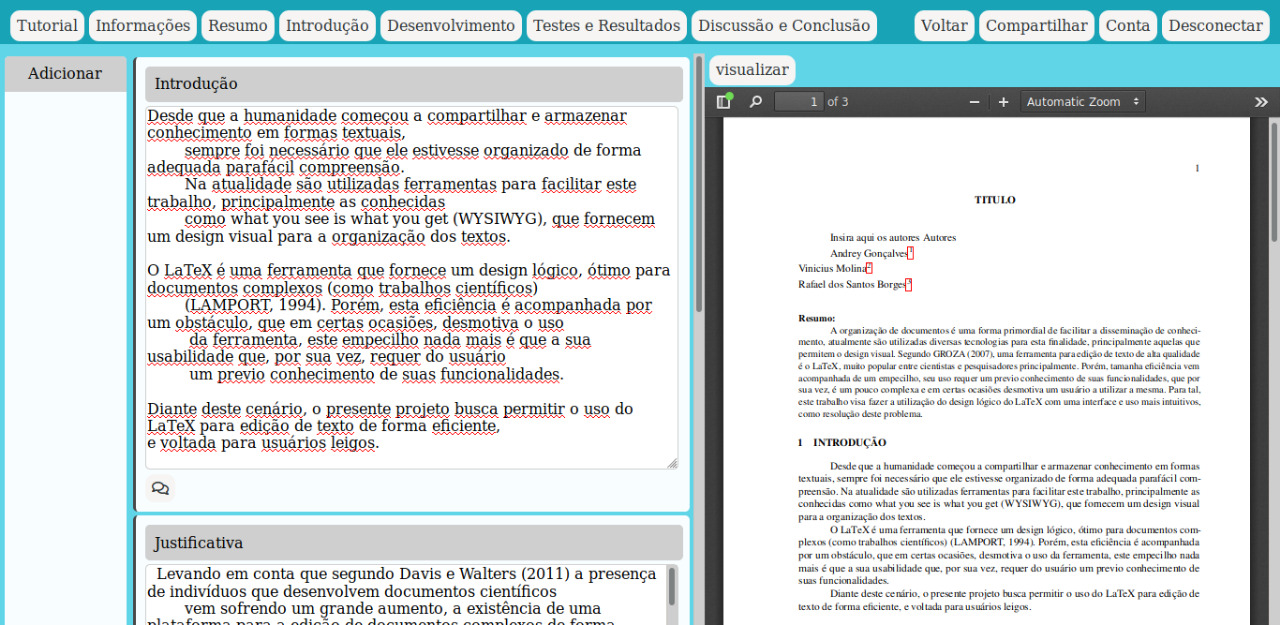
\includegraphics[width=16cm]{figures/Tela Editar Projeto - FATEX.jpeg}
  \textual{Fonte: Dos Autores (2019).}
\end{figure}


A implementação da plataforma base foi inicialmente desenvolvida com Elm, uma linguagem funcional que compila para Java Script, utilizada no desenvolvimento de websites e web apps. Em um momento já avançado do desenvolvimento, notou-se que o mesmo se tornou ineficiente e trabalhoso, devido a certas regras e limitações impostas pela linguagem de programação anteriormente citada.

Como resolução, mesmo com o desenvolvimento já avançado, trocamos o Elm pelo Elixir e seu PHOENIX - LiveView, um framework que permite a implementação de funcionalidades em tempo real, de forma simplificada e performática, sem o uso de Java Script.

A troca se mostrou extremamente positiva, já que ao utilizar os conceitos previamente desenvolvidos em conjunto com a facilidade proporcionada pelo Phoenix – LiveView, conseguimos refazer todo o trabalho de 2 meses em apenas 3 dias, e também resolver nosso problema, ao tornar o desenvolvimento novamente efetivo e simples.

Na integração com banco de dados, foi utilizado o PostgreSQL, e para possibilitar o consumo do mesmo foi utilizado o Phoenix Framework com Elixir.

Para a visualização do PDF com texto formatado em tempo real, foi implementado através do sistema de channels do Phoenix. Para obter o seguinte resultado:


  \begin{figure}[H]
    \centering
    \caption{PDF Renderizado em Tempo Real.}
    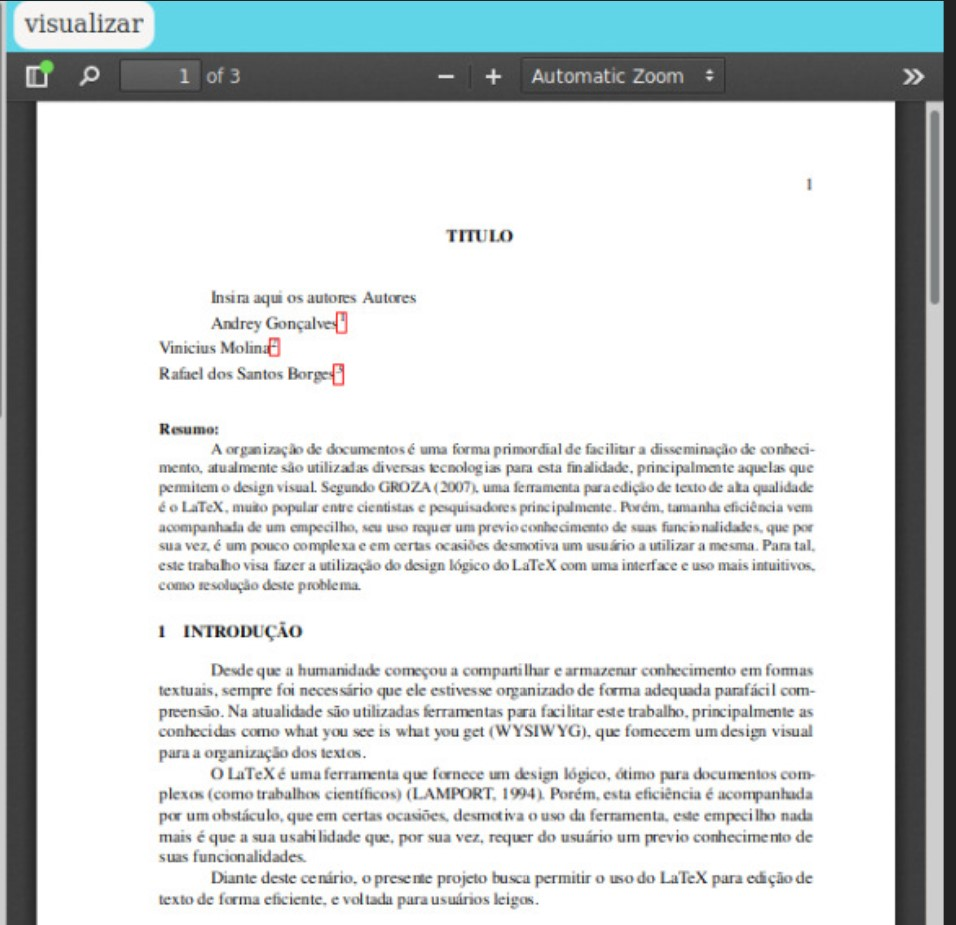
\includegraphics[width=15cm]{figures/PDF Render.jpg}
    \textual{Fonte: Dos Autores (2019).}
  \end{figure}


O projeto possui sistema de Login e autenticação, para que os usuários possam ter seus próprios projetos e compartilhá-los com outras pessoas.


  \begin{figure}[H]
    \centering
    \caption{Tela de Login.}
    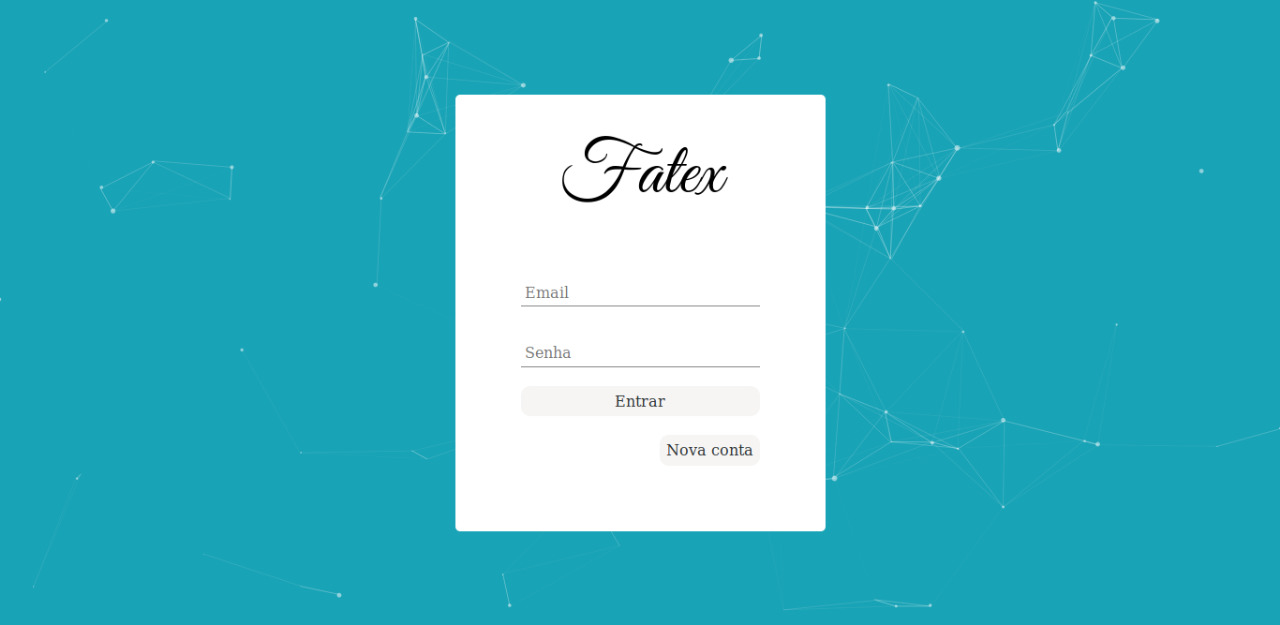
\includegraphics[width=16cm]{figures/Tela Login - FATEX.jpeg}
    \textual{Fonte: Dos Autores (2019).}
  \end{figure}

  \begin{figure}[H]
    \centering
    \caption{Tela de Edição de Cadastro de Usuário.}
    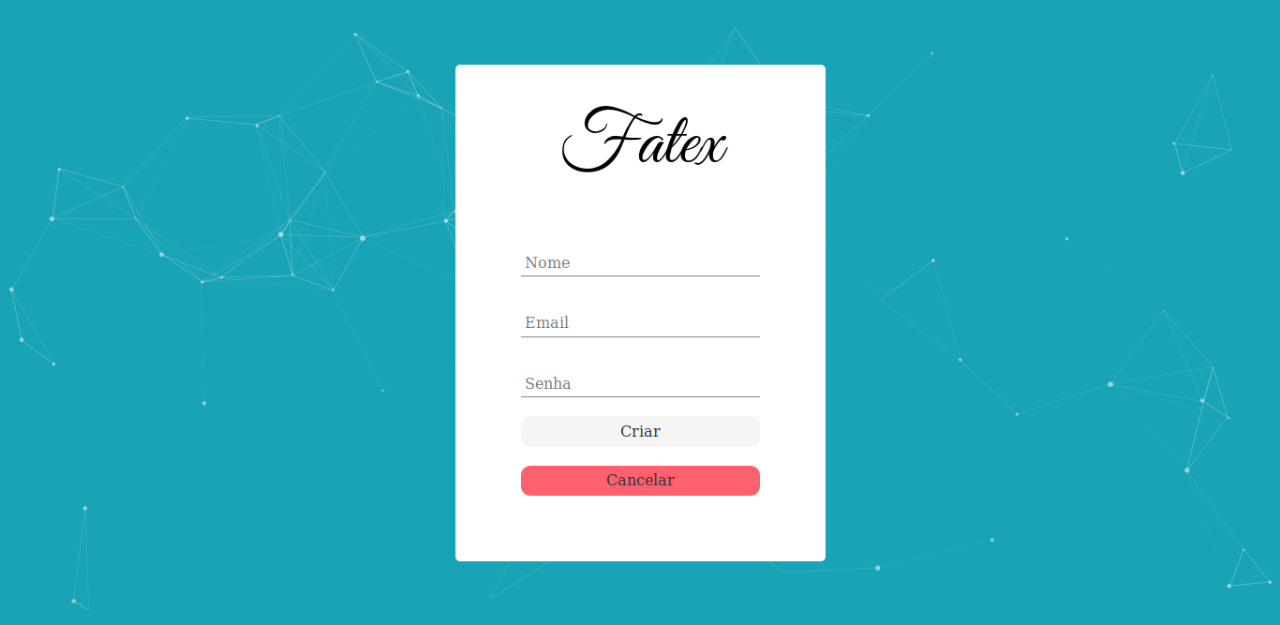
\includegraphics[width=16cm]{figures/Tela Criar Usuario - FATEX.jpeg}
    \textual{Fonte: Dos Autores (2019).}
  \end{figure}


O usuário também pode editar as informações de sua conta.


  \begin{figure}[H]
    \centering
    \caption{Tela de Edição de Edição de Usuário.}
    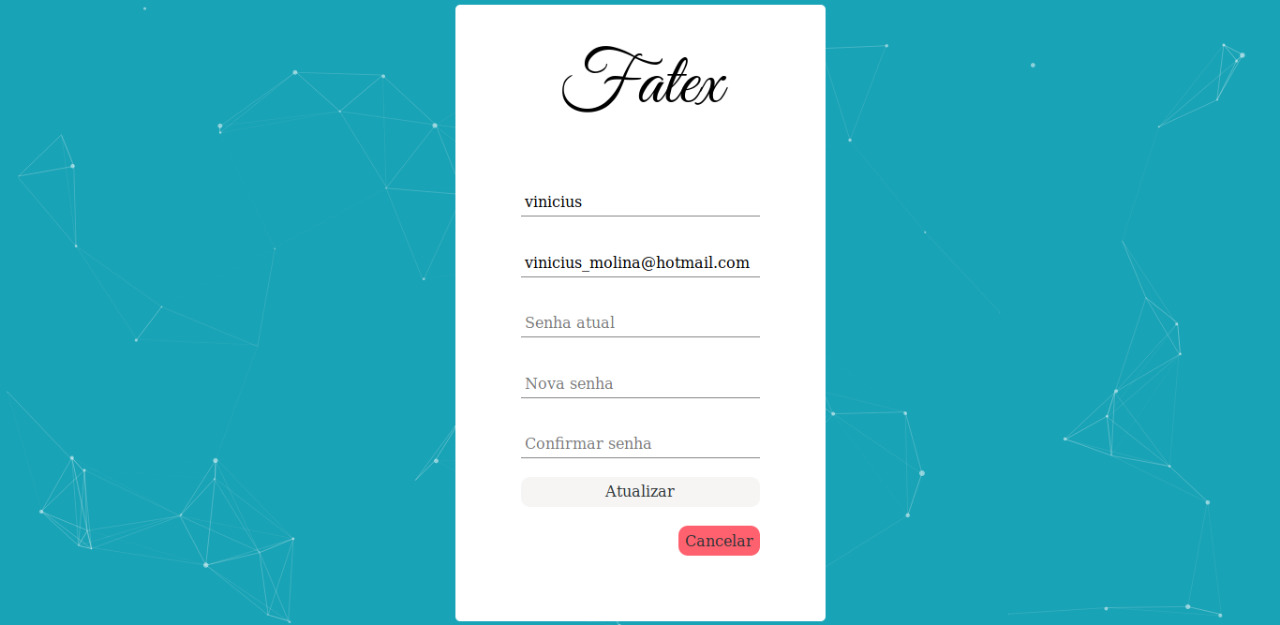
\includegraphics[width=16cm]{figures/Tela Editar Usuario - FATEX.jpeg}
    \textual{Fonte: Dos Autores (2019).}
  \end{figure}


Após fazer login, o usuário tem acesso a todos os seus documentos já desenvolvidos e compartilhados.


  \begin{figure}[H]
    \centering
    \caption{Tela Inicial do Sistema.}
    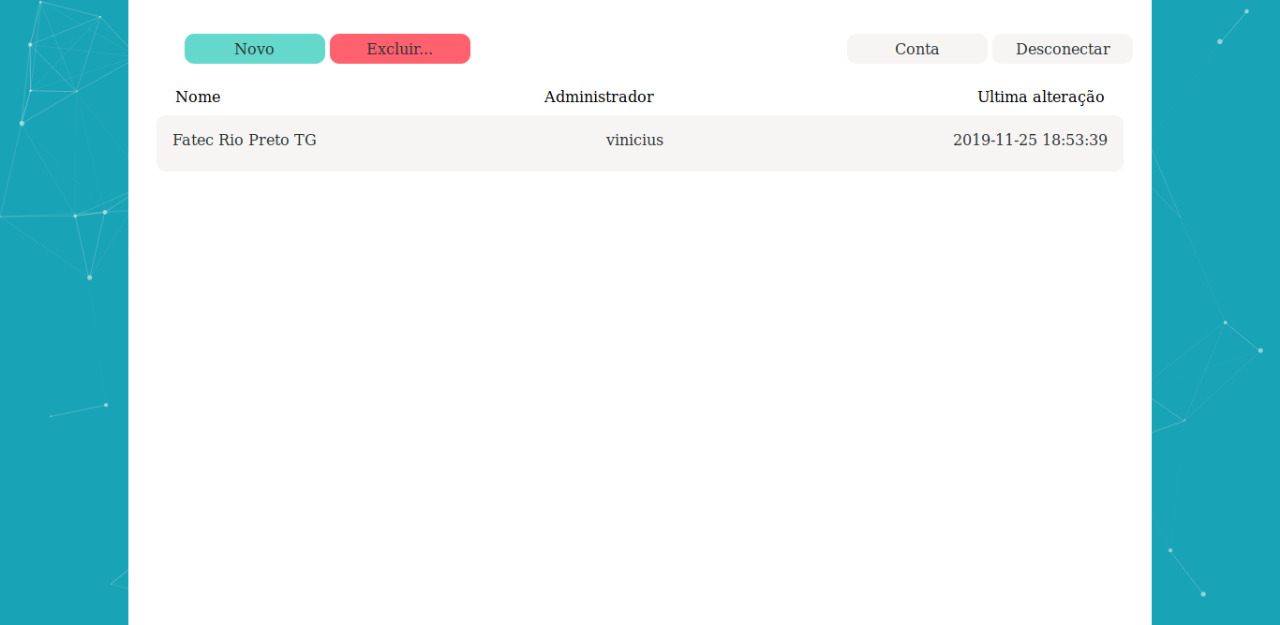
\includegraphics[width=16cm]{figures/Tela Inicial - FATEX.jpeg}
    \textual{Fonte: Dos Autores (2019).}
  \end{figure}


O usuário pode criar documentos definindo nome e template.


  \begin{figure}[H]
    \centering
    \caption{Tela de Criação de Documentos.}
    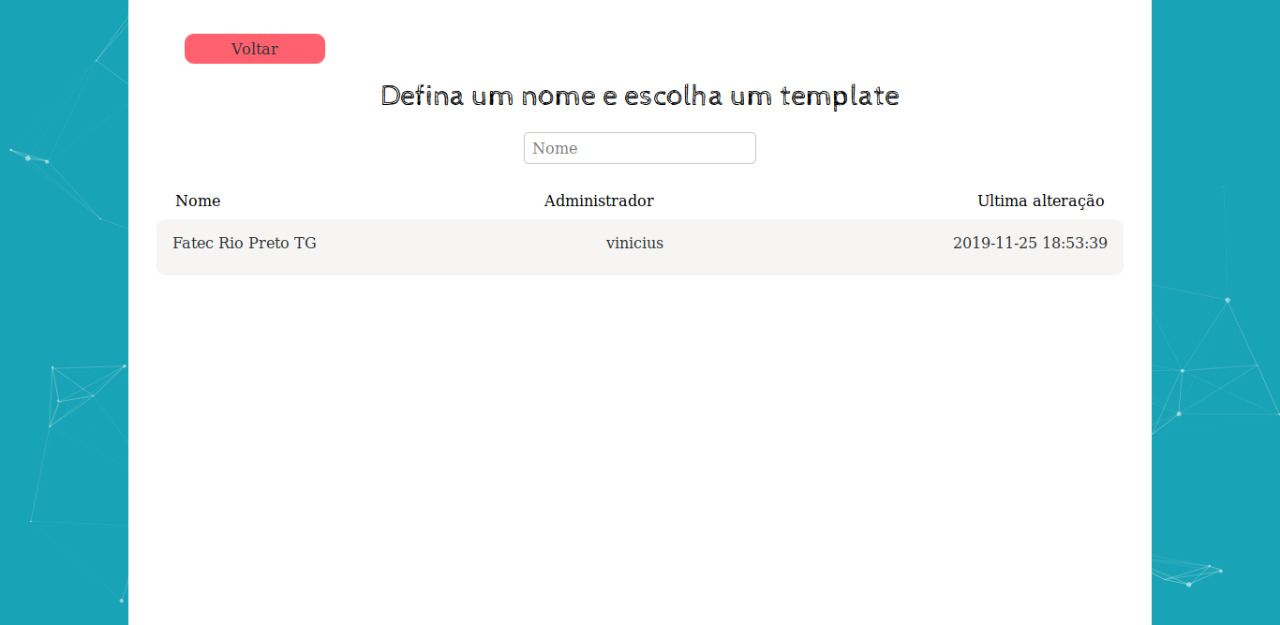
\includegraphics[width=16cm]{figures/Tela Adicionar Projeto - FATEX.jpeg}
    \textual{Fonte: Dos Autores (2019).}
  \end{figure}


Ao abrir um documento ou criar um novo, é exibido um simples tutorial do uso do sistema.


  \begin{figure}[H]
    \centering
    \caption{Tela Inicial dos Documentos.}
    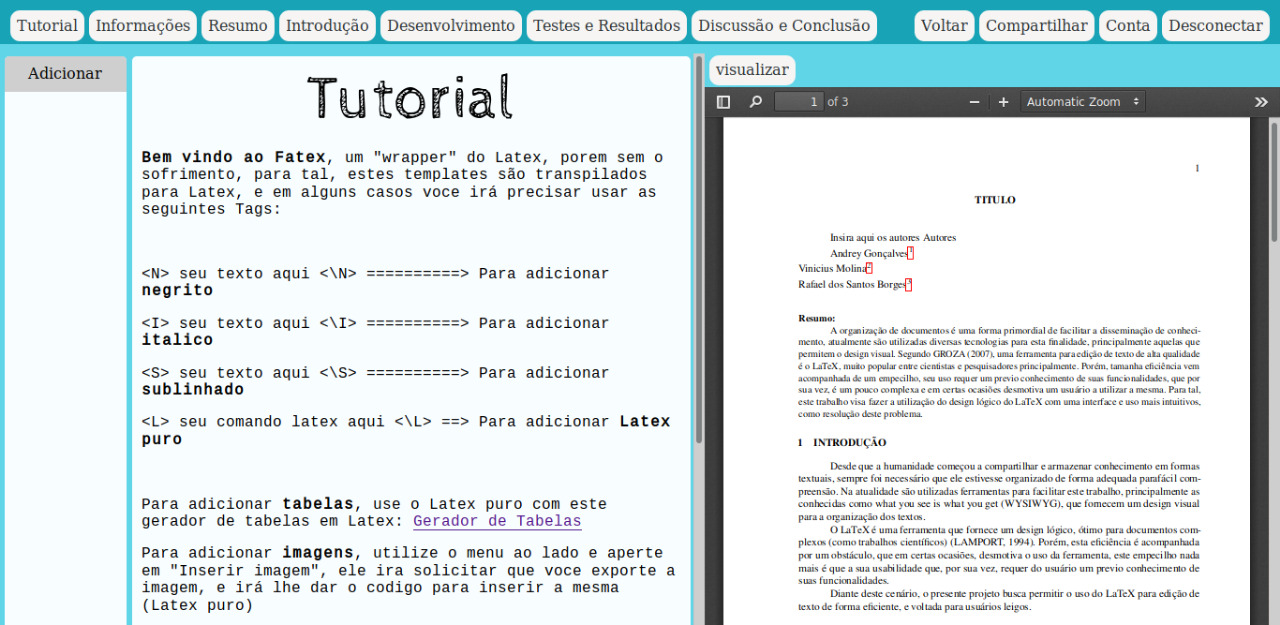
\includegraphics[width=16cm]{figures/Tela Inicial do Projeto - FATEX.jpeg}
    \textual{Fonte: Dos Autores (2019).}
  \end{figure}

  \begin{figure}[H]
    \centering
    \caption{Tela de Edição de Documentos.}
    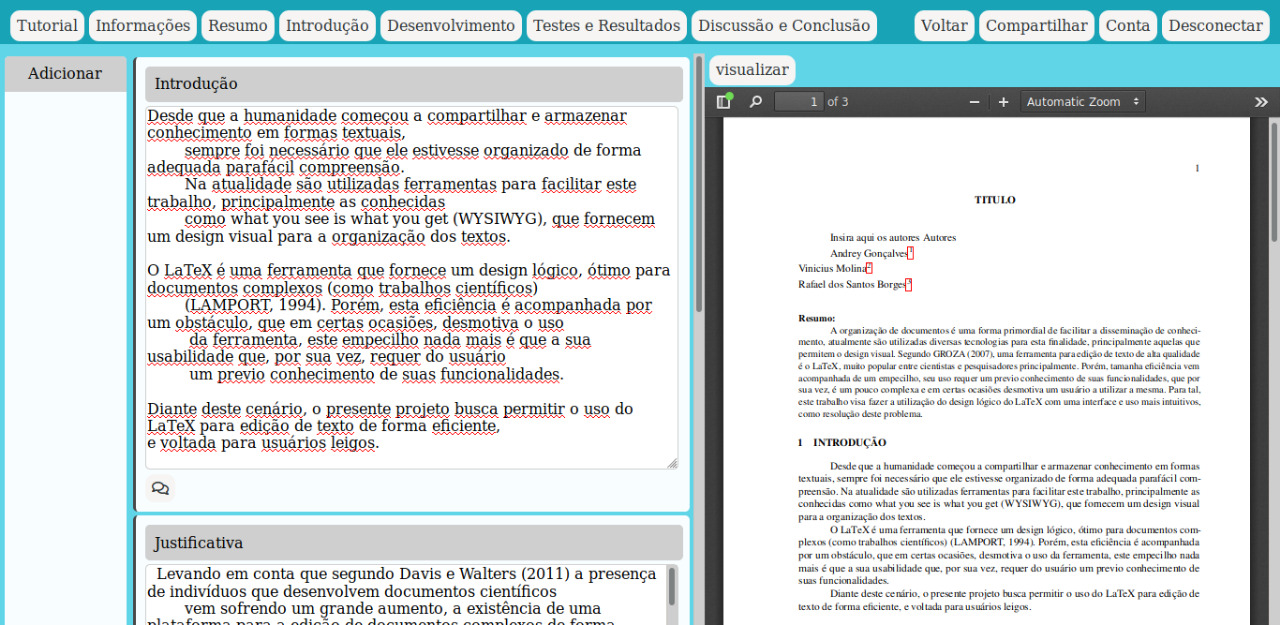
\includegraphics[width=16cm]{figures/Tela Editar Projeto - FATEX.jpeg}
    \textual{Fonte: Dos Autores (2019).}
  \end{figure}


Também é possível compartilhas seus documentos com outros usuários permitindo-os editar e comentar.


  \begin{figure}[H]
    \centering
    \caption{Tela de Compartilhamento.}
    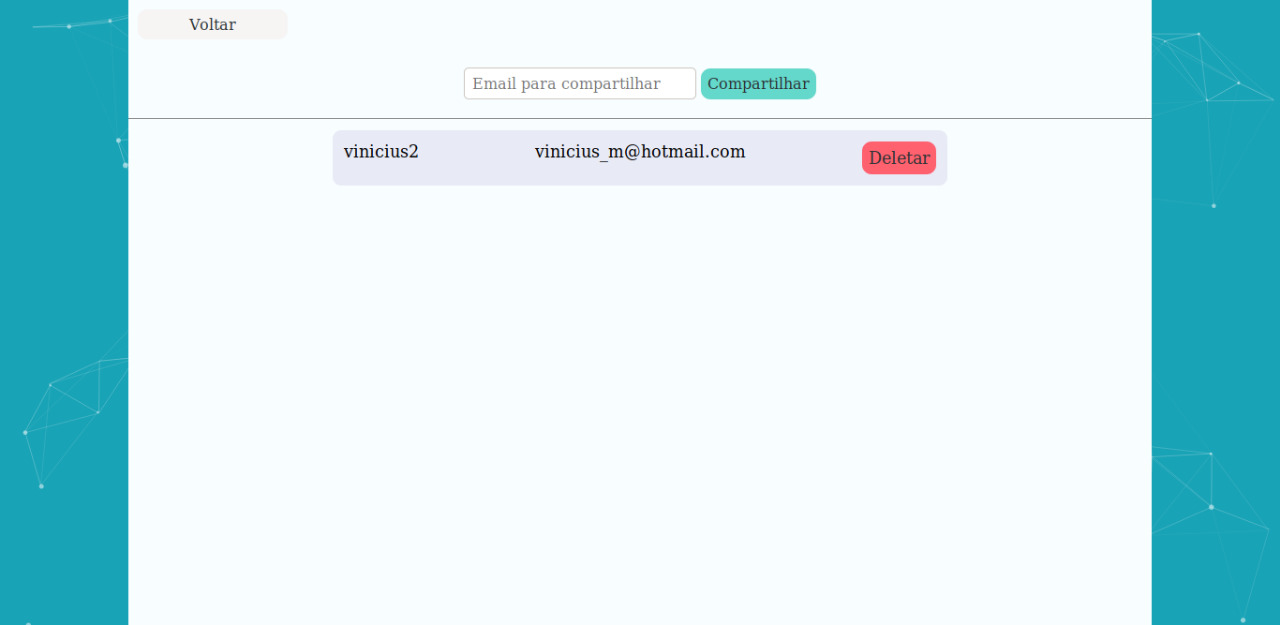
\includegraphics[width=16cm]{figures/Tela Compartilhar Projeto - FATEX.jpeg}
    \textual{Fonte: Dos Autores (2019).}
  \end{figure}






\section{Resultados e Discussões}

Resultados Resultados Resultados Resultados Resultados Resultados Resultados Resultados Resultados Resultados Resultados Resultados Resultados.





\section{Conclusões}

Conclusões Conclusões Conclusões Conclusões Conclusões Conclusões Conclusões Conclusões Conclusões Conclusões Conclusões Conclusões Conclusões.





\section{Referências}
\raggedright


BRACHET, Pascal. \textbf{TEXMARKER: Free cross-platform LaTeX editor since 2003.} [S. l.], 2003 - 2019. Disponível em: https://www.xm1math.net/texmaker/download.html. Acesso em: 10 jul. 2019.

DAVIS, Philip M.; WALTERS, William H. \textbf{The impact of free access to the scientific literature: a review of recent research.} Journal of the Medical Library Association: JMLA, v. 99, n. 3, p. 208, 2011.

DEBENEDETTO, Sophie. \textbf{Walk-Through of Phoenix LiveView: What is LiveView?} [S. l.], 19 mar. 2019. Disponível em: https://elixirschool.com/blog/phoenix-live-view/. Acesso em: 20 out. 2019.

DONALD, E. K. \textbf{The TEXbook, volume A of Computers and Typesetting.} [S. l.]: Addison-Wesley, Reading, Massachusetts” 1989.

GROZA, Tudor et al. \textbf{SALT-Semantically Annotated {LaTeX} for Scientific Publications.} In: European Semantic Web Conference. Springer, Berlin, Heidelberg, 2007. p. 518-532.

GOOGLE PLAY. \textbf{VerbTeX LaTeX Editor.} [S. l.], 2 abr. 2019. Disponível em: https://play.google.com/store/apps/details?id=verbosus.verbtex&hl=pt-BR. Acesso em: 20 maio 2019a.

GOOGLE PLAY. \textbf{NeutriNote.} [S. l.], 8 jun. 2019. Disponível em: https://play.google.com/store/apps/details?id=com.appmindlab.nano. Acesso em: 24 jun. 2019b.

GOOGLE PLAY. \textbf{LawTeX.} [S. l.], 12 dez. 2018. Disponível em: https://play.google.com/store/apps/details?id=law.tex. Acesso em: 24 jun. 2019c.

GOOGLE PLAY. \textbf{TeX Writer - LaTeX On the Go.} [S. l.], 28 nov. 2017. Disponível em: https://play.google.com/store/apps/details?id=com.litchie.texwriter. Acesso em: 24 jun. 2019d.

LAMPORT, L. \textbf{LATEX: a document preparation system: user’s guide and reference manual.} [S. l.]: Addison-wesley, 1994.

MARCIAL, E. C. O. \textbf{Megatendências mundiais 2030: o que entidades e personalidades internacionais pensam sobre o futuro do mundo?: contribuição para um debate de longo prazo para o brasil.} Instituto de Pesquisa Econômica Aplicada (Ipea), 2015.

THE POSTGRESQL GLOBAL DEVELOPMENT GROUP. \textbf{PostgreSQL: The World‘s Most Advanced Open Source Relational Database: New to PostgreSQL?.} [S. l.], 2019. Disponível em: https://www.postgresql.org/. Acesso em: 18 ago. 2019.

MUNDIAL, B. \textbf{Relatório sobre o desenvolvimento mundial de 2012, visão geral: Igualdade de gênero e desenvolvimento.} Washington: Banco Internacional de Reconstrução e Desenvolvimento e Banco Mundial, 2011.

PLATAFORMATEC. \textbf{Elixir.} [S. l.], 2019. Disponível em: https://elixir-lang.org/. Acesso em: 1 nov. 2019.

OETIKER, T. et al. \textbf{The not so short introduction to latex 2.} Or LATEX 2d in, Citeseer, v. 69, 2011.

SUTHERLAND, J. \textbf{Scrum: a arte de fazer o dobro do trabalho na metade do tempo.} [S. l.]: Leya, 2016.

ZANDER, Benito van der. \textbf{TeXstudio: LaTeX made comfortable. 2.12.16.} [S. l.], 19 maio 2019. Disponível em: https://www.texstudio.org/. Acesso em: 11 jul. 2019.
ZIEGELMAYER, Friedel. \textbf{Argon2_elixir: Argon2. 2.1.2.} [S. l.], 2019. Disponível em: https://hexdocs.pm/argon2-elixir/Argon2.html. Acesso em: 20 nov. 2019.


\end{document}



